% Pdf only
\documentclass[aspectratio=169]{beamer}
% For presentation
%\documentclass[aspectratio=169, notes]{beamer}
\usepackage{lmodern}
\usepackage{pgfpages}
%\setbeameroption{show notes on second screen}
%\usepackage[utf8]{inputenc} 
\usepackage[english]{babel}

%
% Choose how your presentation looks.
%
% For more themes, color themes and font themes, see:
% http://deic.uab.es/~iblanes/beamer_gallery/index_by_theme.html
%
\mode<presentation>
{
  \usetheme[]{metropolis}           % Use metropolis theme
} 

\begin{document}
\obeylines

\title[ORB SLAM Point Cloud generation on Apalis iMX8]{ORB SLAM Point Cloud generation on Apalis iMX8}
\author{Stefan Eichenberger, CPVR Lab}
\date{25.01.2019}


\begin{frame}
  \titlepage\thispagestyle{empty}
\end{frame}

\note[itemize]{
\item Herzlich wilkommen zur Präsentation über ORB Slam Point Cloud generation on Apalis iMX8
\item Wer von euch hat zuhause einen Staubsaugerroboter?
\item Wer findet der ist super intelligent?
}

\begin{frame}{Why SLAM}
  \begin{center}
    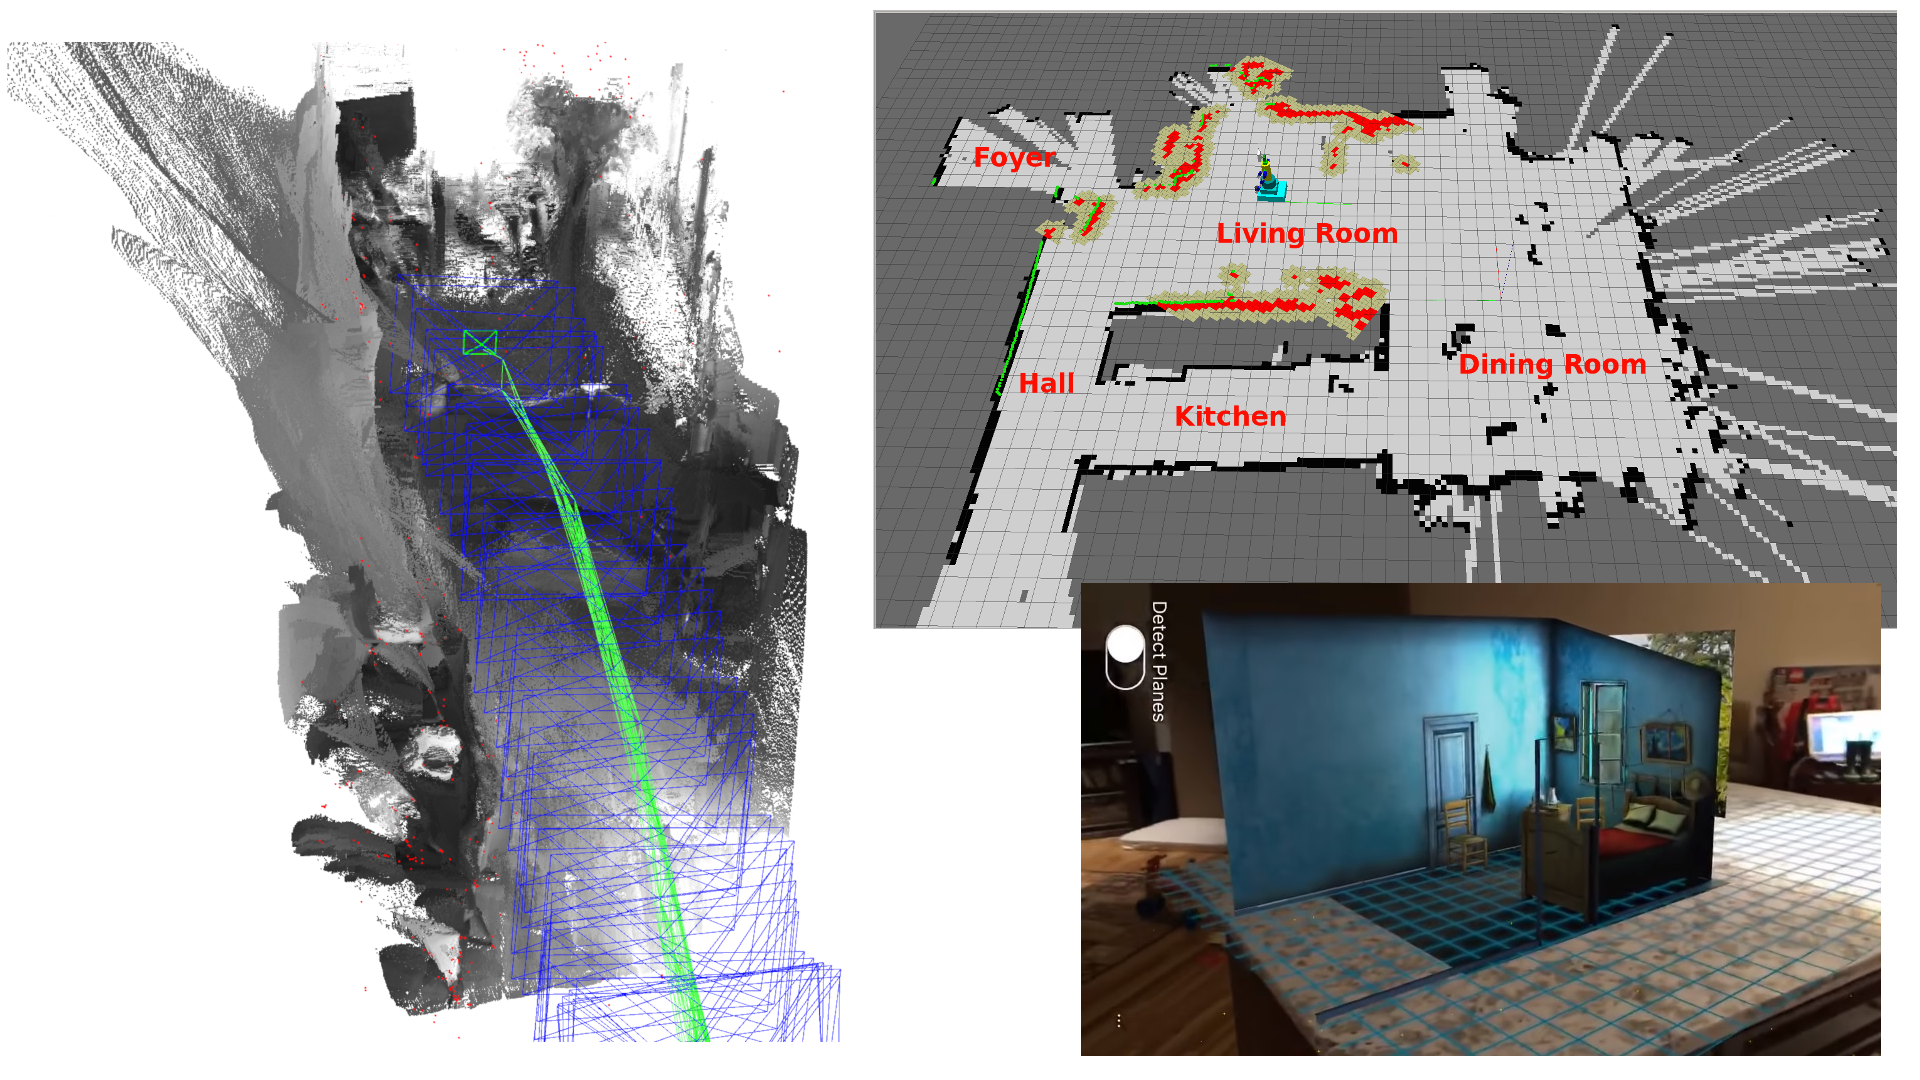
\includegraphics[height=0.9\textheight]{./img/slam_usecases.png}
  \end{center}
\end{frame}

\note{
}

\begin{frame}{Toradex Apalis iMX8}
  \begin{center}
    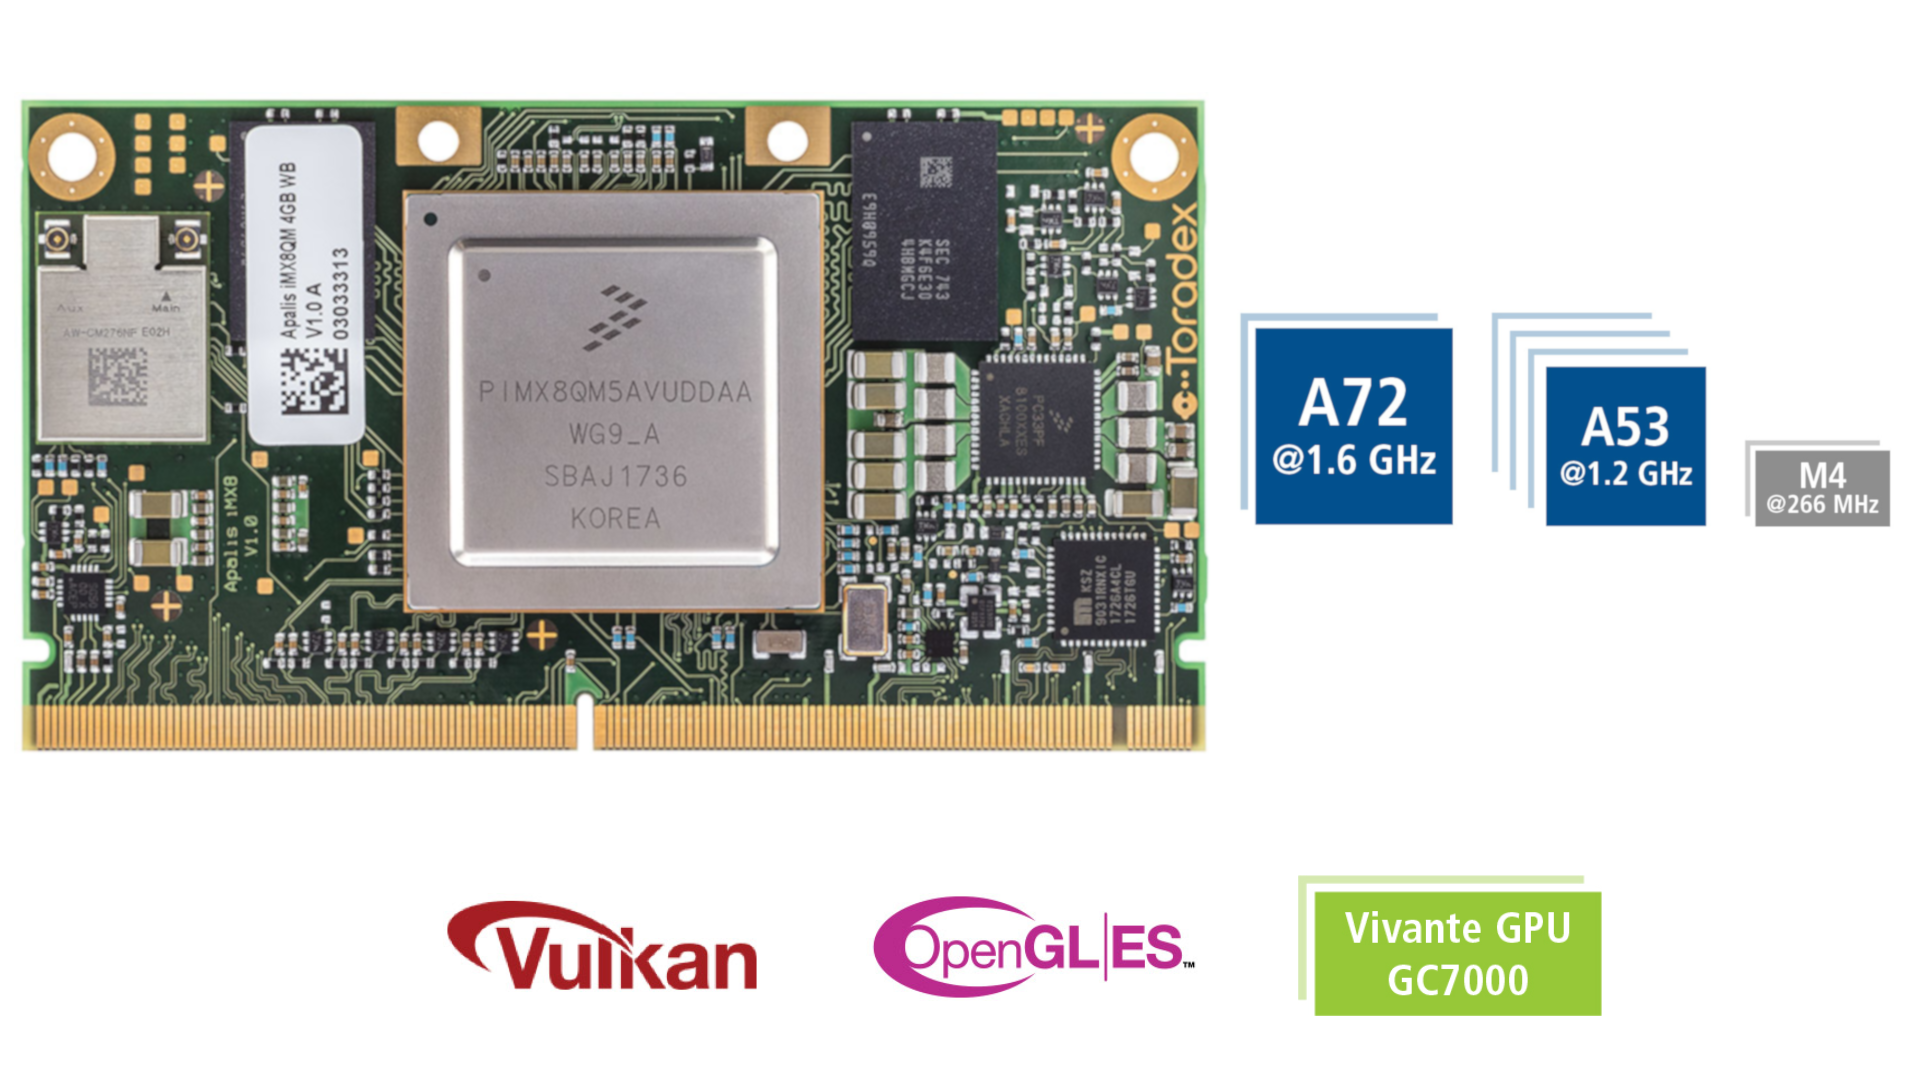
\includegraphics[height=0.9\textheight]{./img/apalis_imx8_slide.png}
  \end{center}
\end{frame}

\note{
}

\begin{frame}{Why Apalis iMX8?}
  \begin{center}
    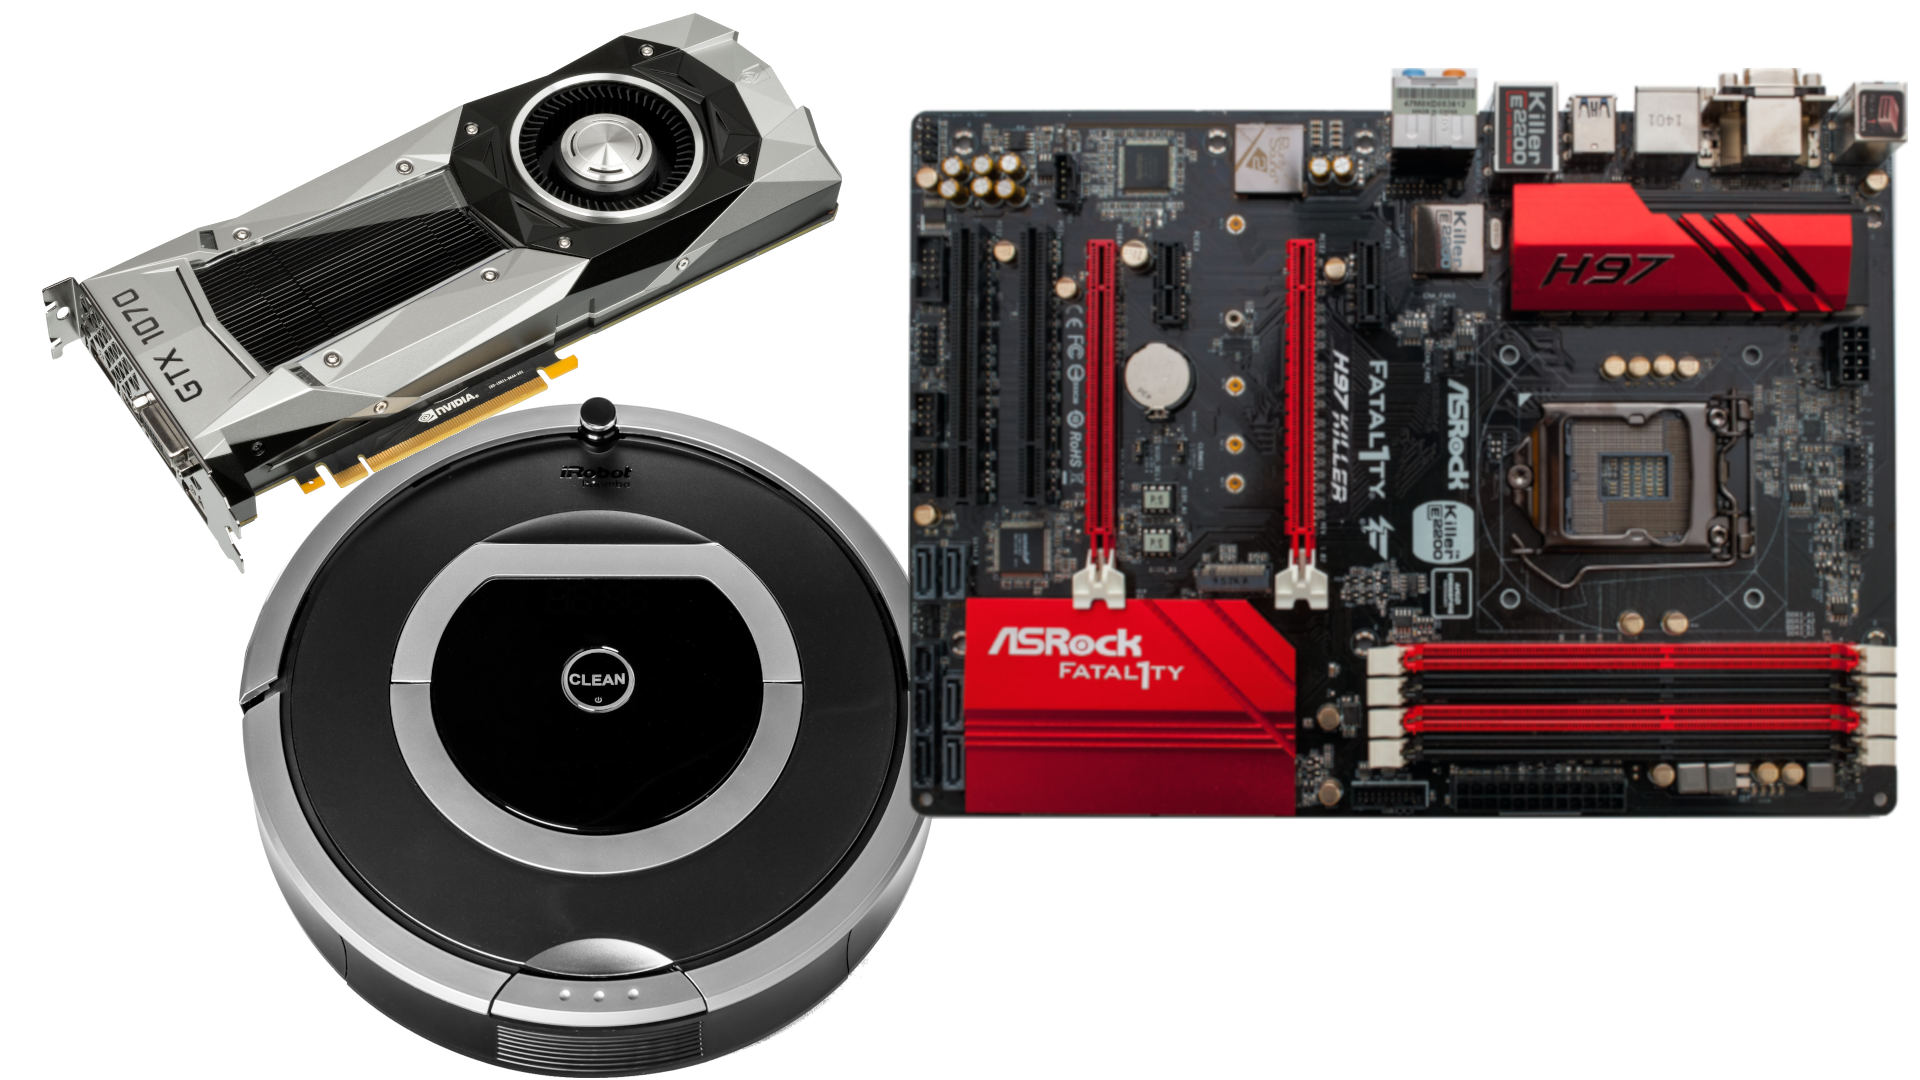
\includegraphics[height=0.9\textheight]{./img/robot_size.png}
  \end{center}
\end{frame}

\note{
}

\begin{frame}{Stereo Camera}
  \begin{center}
    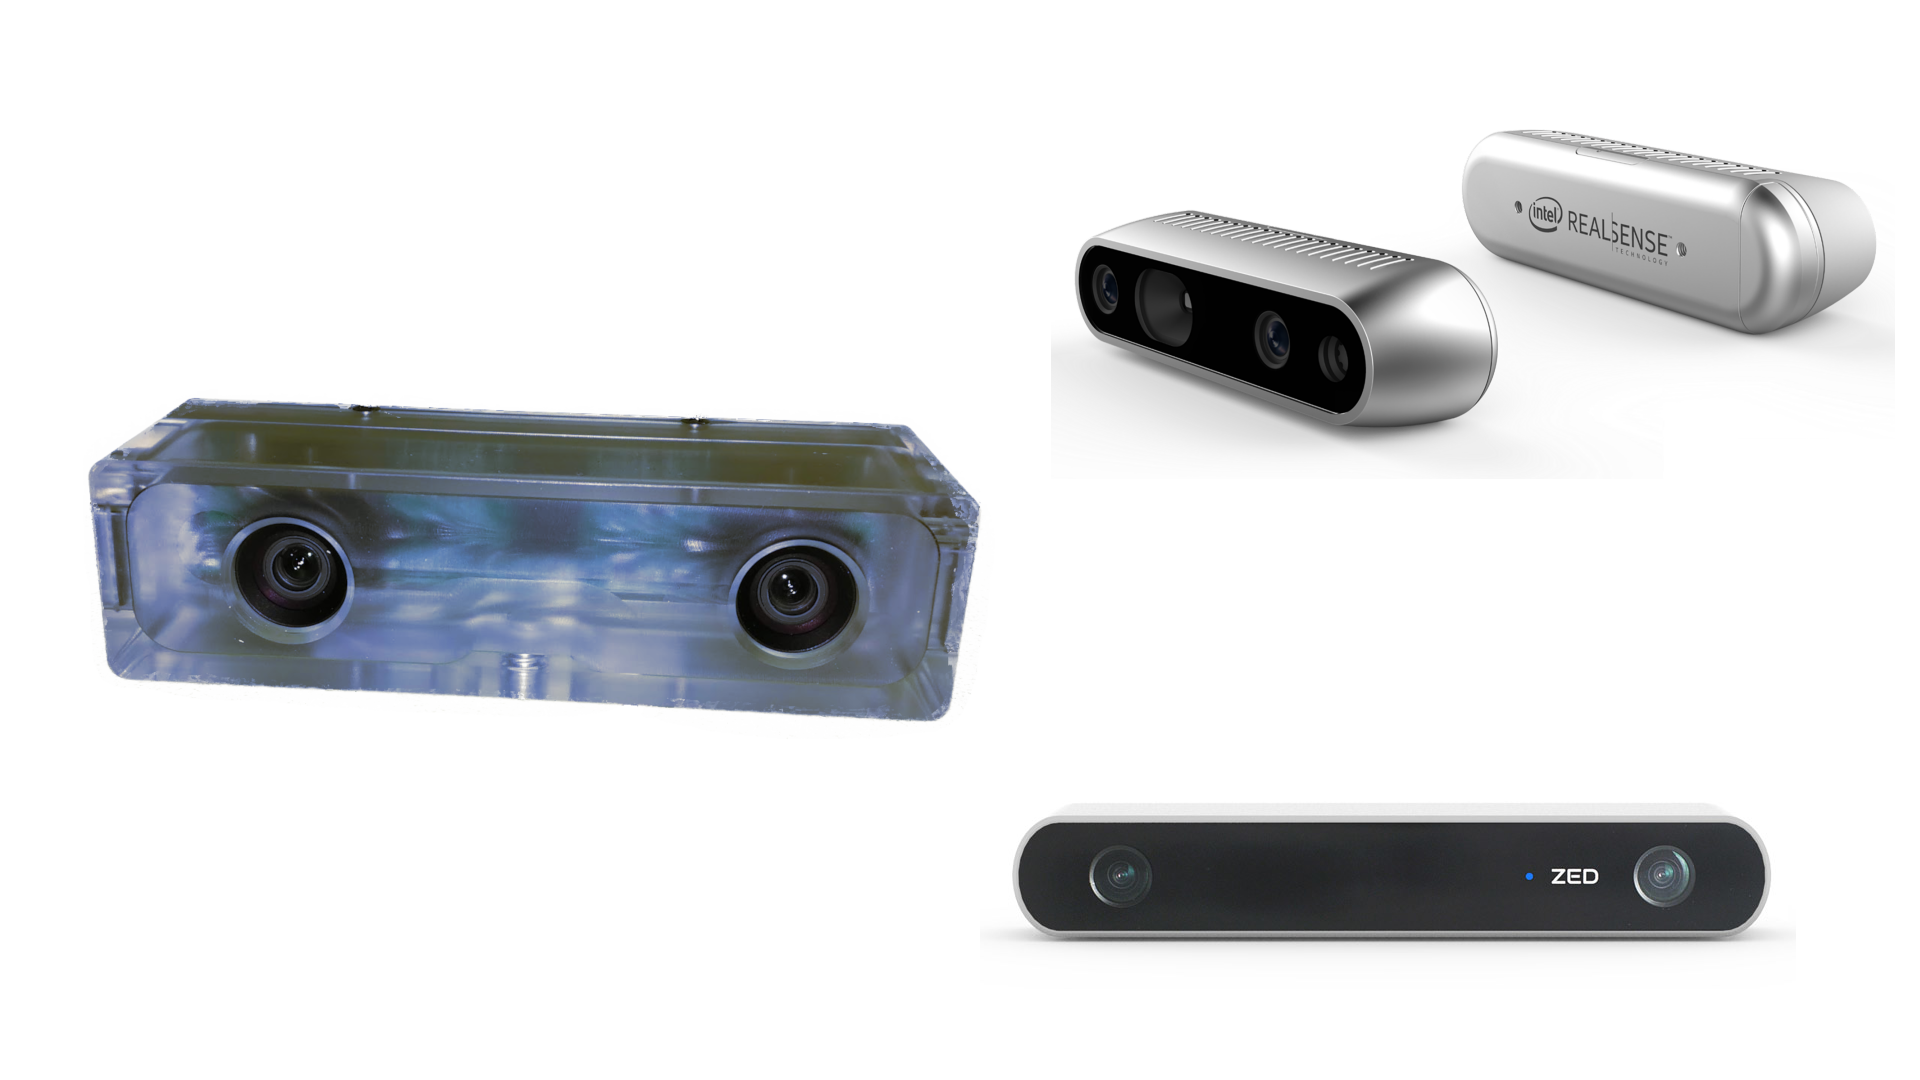
\includegraphics[height=0.9\textheight]{./img/cameras.png}
  \end{center}
\end{frame}

\note{
}


\begin{frame}{Stereo Calibration}
  \begin{center}
    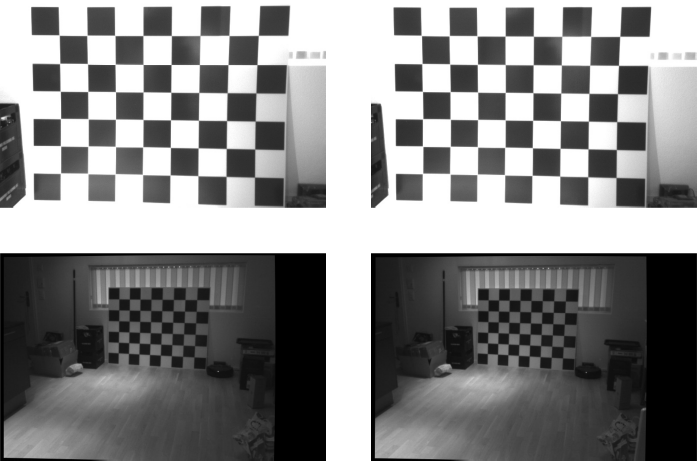
\includegraphics[height=0.9\textheight]{./img/stereo_calib.png}
  \end{center}
\end{frame}

\note{
}

%\begin{frame}{Stereo SLAM}
%  \begin{center}
%    \includegraphics[height=0.9\textheight]{./img/fixar.jpg}
%  \end{center}
%\end{frame}
%
%\note{
%}

\begin{frame}{Different SLAMs}
  \begin{center}
    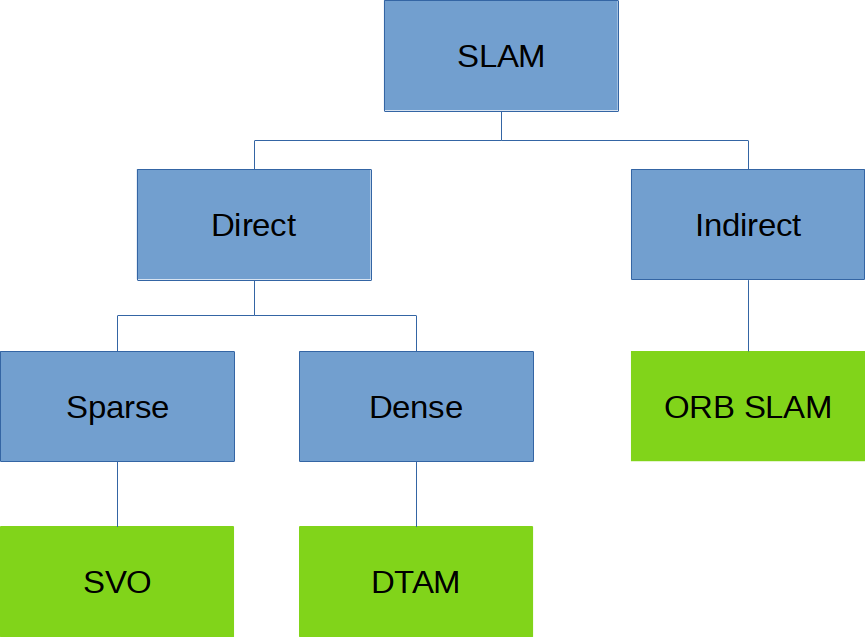
\includegraphics[height=0.9\textheight]{./img/slam_modes.png}
  \end{center}
\end{frame}

\note{
}

%\begin{frame}{ORB SLAM}
%  \begin{center}
%    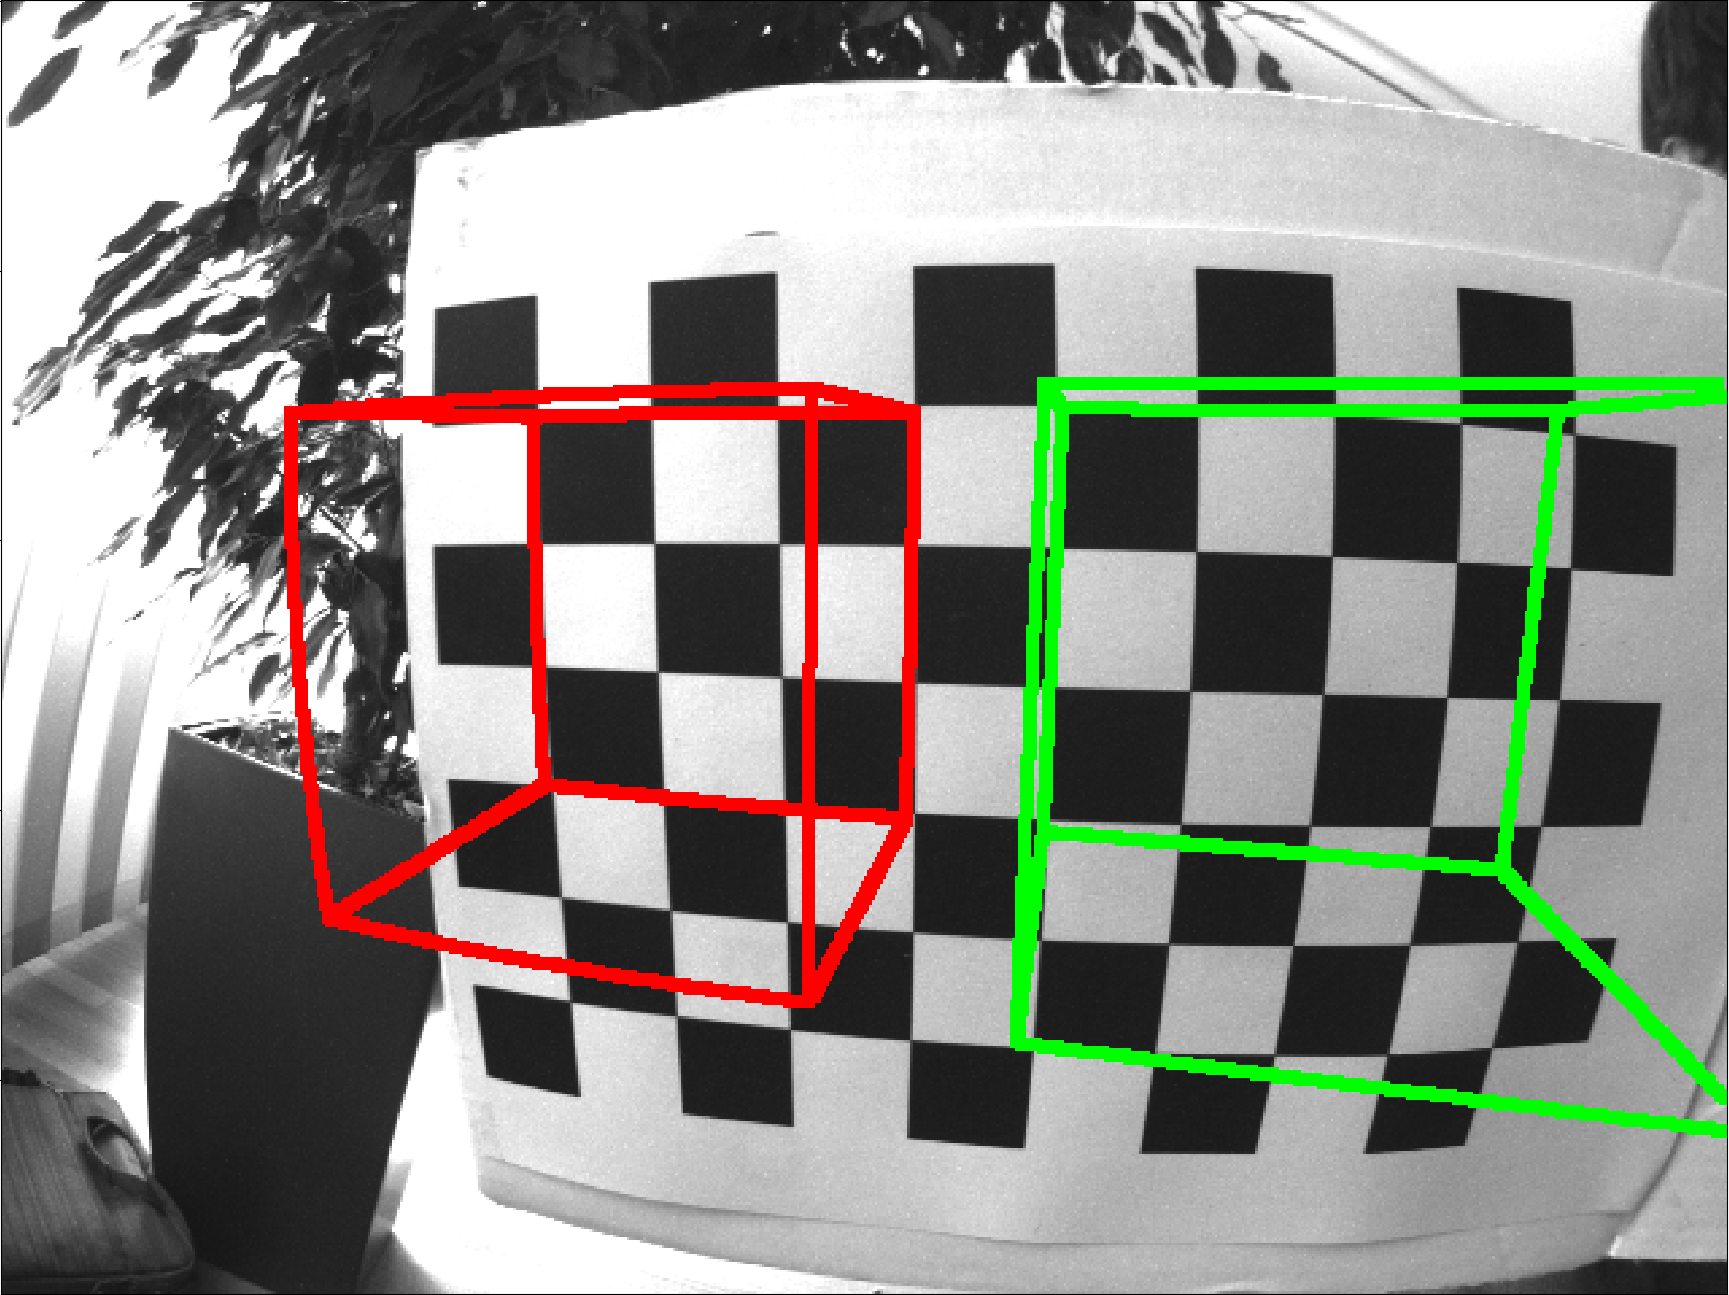
\includegraphics[height=0.9\textheight]{./img/model.png}
%  \end{center}
%\end{frame}
%
%\note{
%}
%
%\begin{frame}{Densification}
%  \begin{center}
%    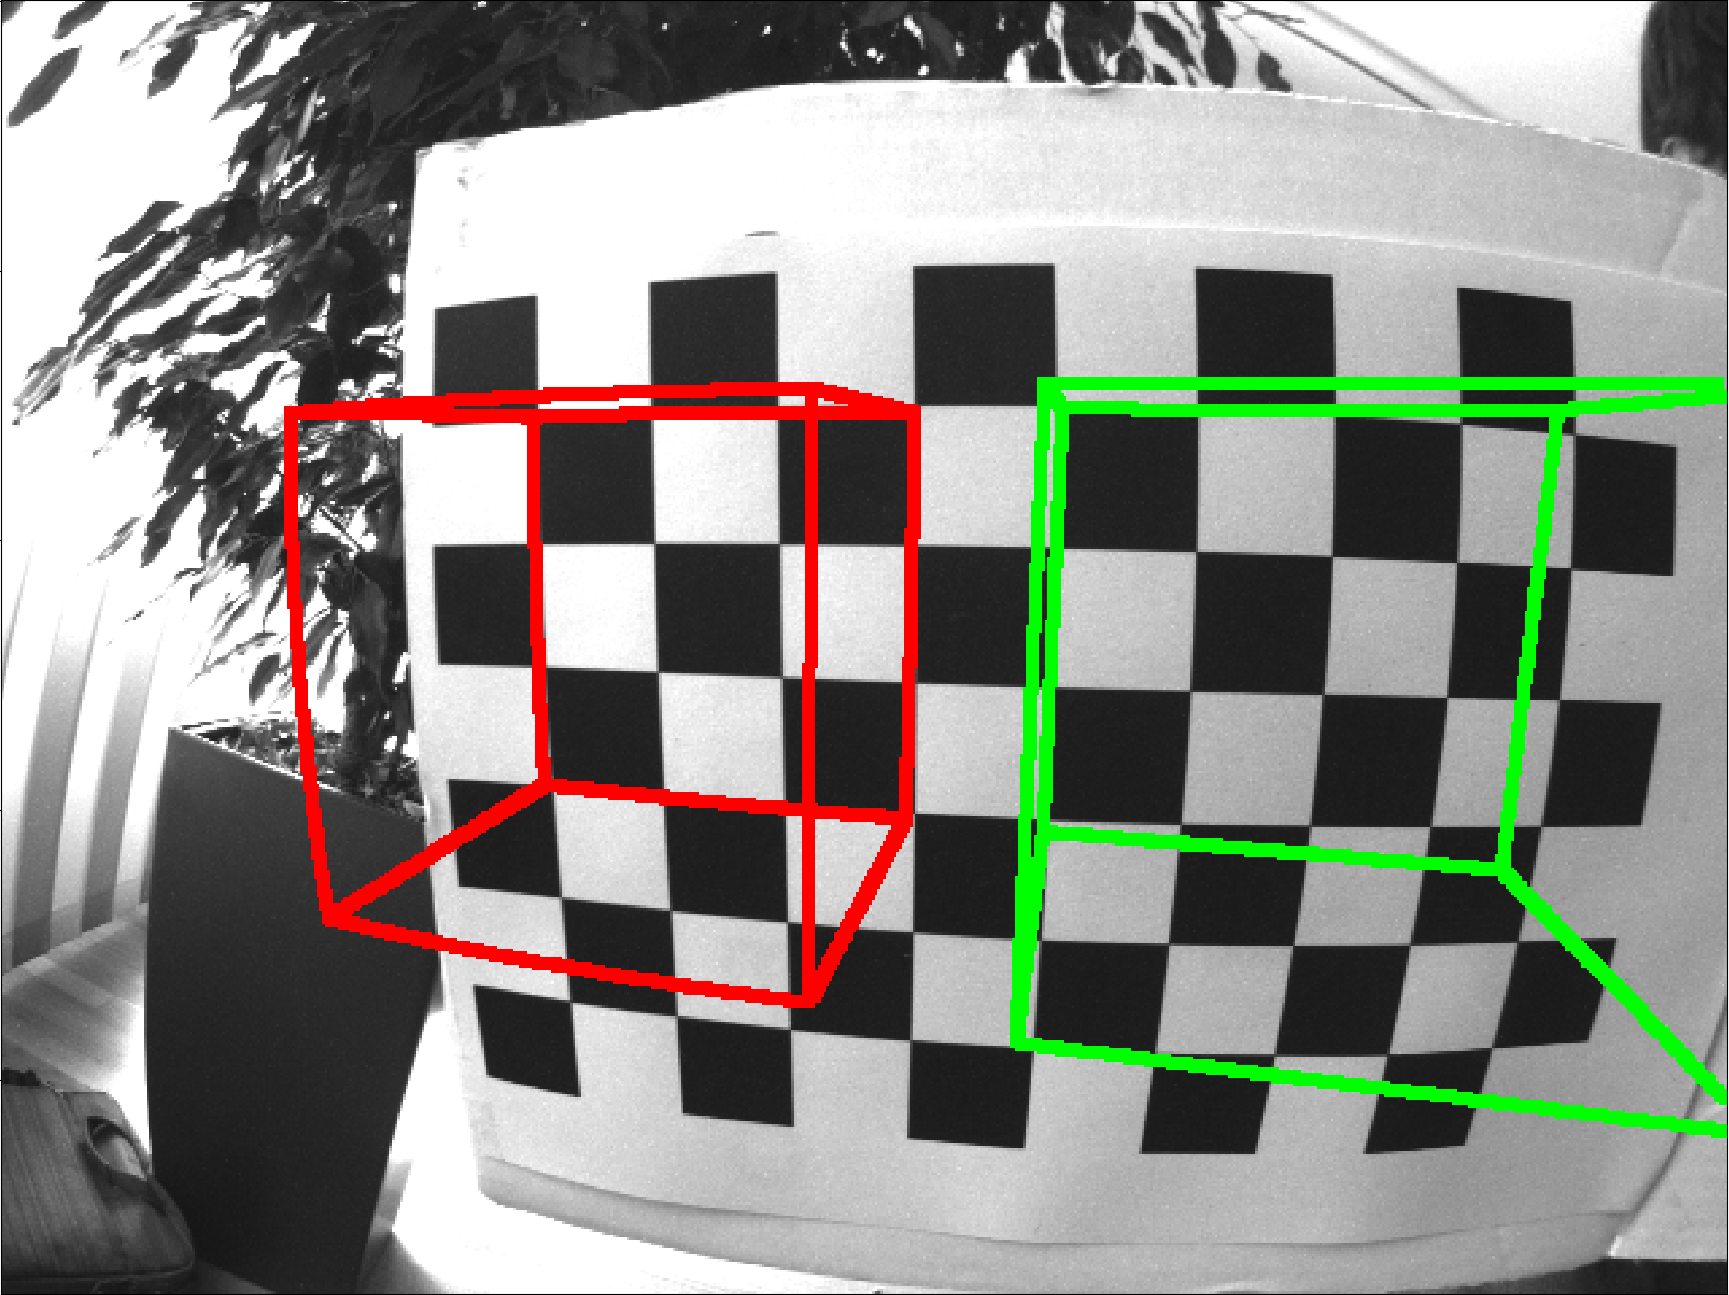
\includegraphics[height=0.9\textheight]{./img/model.png}
%  \end{center}
%\end{frame}
%
%\note{
%}
%
%\begin{frame}{Results}
%  \begin{center}
%    \includegraphics[height=0.9\textheight]{./img/chess_calibration.jpg}
%  \end{center}
%\end{frame}
%
%\note{
%}
%
%\begin{frame}{Demo}
%  \begin{center}
%    \includegraphics[height=0.9\textheight]{./img/chess_calibration.jpg}
%  \end{center}
%\end{frame}
%
%\note{
%}
%
%\begin{frame}{Direct Approach}
%  \begin{center}
%    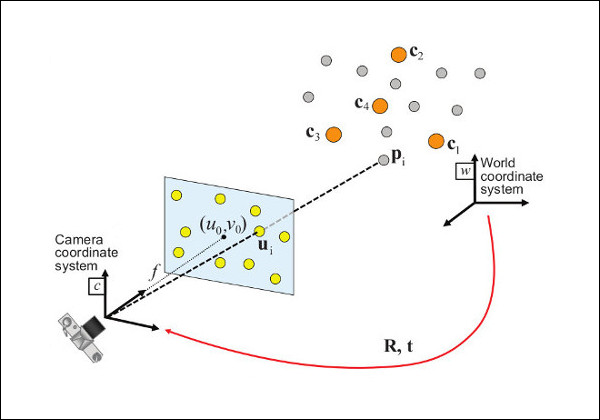
\includegraphics[height=0.9\textheight]{./img/pnp.jpg}
%  \end{center}
%\end{frame}
%
%\note{
%}
%
%\begin{frame}{Questions}
%  \begin{center}
%    
\includegraphics[height=0.9\textheight]{./img/question.jpg}
%  \end{center}
%\end{frame}


\end{document}

